\section{Background and Related Works}
\label{sec:related}
Epidemic models are used to predict the progression of infectious diseases in a given population and the likely outcome of an epidemic. 
%The existing spectrum ranges from coarse population-based models to detailed agent-based models. 
The classical susceptible-infected-susceptible (SIS) model depicted in \figurename{~\ref{figure:sis}} serves as the basis for many extended models, wherein $S_i(t)$ and $I_i(t)$ denote the probability of node $i$ being in the susceptible ($S$) or the infected ($I$) state, respectively, in a network of size $N$ \cite{Vynnycky2010}. Nodes that recover from the infection immediately transition to being susceptible again. The discrete-time node-level SIS epidemic model has the following form:
\begin{align}
	S_i(t) = \beta S_i(t-1) \sum_{j=1}^N a_{i,j} p_j(t) - \gamma p_i(t),
\end{align} 
satisfying the condition $S_i(t) + I_i(t) = 1$ for all $t$ values. Here, $\beta$ denotes the rate at which node $i$ gets infected, $\gamma$ is the recovery rate, $p_i$ is the probability of $i$ being infected at time $t$, and $a_{ij}$ is any element in the adjacency matrix $A$ corresponding to the network defined as:
\begin{align}
    A =\! \{a_{ij}\} \!=\! 
\begin{cases}
    1,   & \text{if } \text{nodes \emph{i} and \emph{j} are connected neighbors}\\
    0,   & \text{otherwise}.
\end{cases}
\end{align}

Advancements in network science led to the revival of several unique recurring patterns inherent in networks which essentially drive the spreading pattern of processes. The Erd\"{o}s-R\'{e}nyi (ER) model was the first to be used for generating typical random networks \cite{Erdos60onthe}. 
%Although having limited realistic applications, the model serves as a benchmark for many studies due to its interesting characteristics. 
An ER network of $N$ nodes, wherein a link is included independent of other links with probability $p$, has a mean link count of $\binom{N}{2} p$, mean degree of $(N-1)p$, and binomial degree distribution. Such networks manifest low degree heterogeneity (most nodes have the same degree), low clustering coefficient (probability that two neighbors of a node are also neighbors), and short average path length.
While ER networks are highly robust against deliberate attacks, they lack the large degree of transitivity witnessed in reality. To overcome this shortcoming, the Watts-Strogatz (WS) model was proposed to generate random graphs with small-world properties by rewiring the links of a lattice with some given probability \cite{barabasi2016network}.
This model is built on the interpolation between a standard ER random graph and a network with maximal clustering.
The Barab\'{a}si-Albert (BA) model was then developed to generate random scale-free networks with high degree heterogeneity. Based on the concept of preferential attachment or ``the rich gets richer'', the network initially begins with at least two nodes where a newly added node is most likely to connect to nodes with higher degrees. This results in the formation of a few highly-connected nodes in the network. The resulting network degree distribution has no characteristic scale as they have power law tail. Unlike ER networks that exhibit an average distance of $\log(n)$, scale-free BA networks are ultra small-world networks with a sub-logarithmic small diameter proportional to $\log(\log(n))$ and thus, are particularly robust against random node failures.

\begin{figure}[!t]
    \begin{center}
    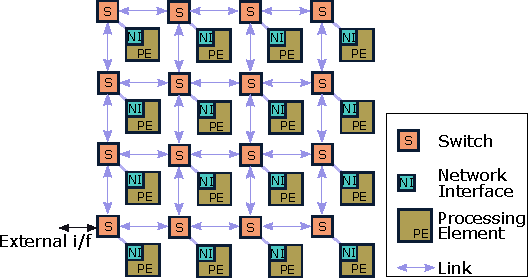
\includegraphics[width=0.6\columnwidth]{Figures/noc.pdf}
    \caption{Proposed NoC-based platform with mesh topology showing switch interconnections and network interfaces.} 
    \label{figure:noc}
    \end{center}
    \vspace{-8mm}
\end{figure}


Except for a few, most of the existing simulation tools support deterministic modeling of simplified processes. EpiModel \cite{Jenness2018} is an R package to analyze stochastic individual and network-level epidemic models. A stochastic simulator for generalized epidemic modeling known as GEMFsim \cite{SAHNEH201736} has been reported and made available in MATLAB, R, Python, and C programming platforms. These simulators however, demand longer running time as the scale and complexity of the network increases.
%\todo[inline]{If possible please shorten the description of different network models and fit into a single para. Rather explain why these different models are significant in modeling. Also a few lines on the traditional approach of modeling, like they are modeled using modeling software such as Matlab and Simulink. This might give a motivation to apply hardware acceleration.}

In this work, we propose to emulate the SIS process on an NoC platform.
NoC is an interconnect approach that helps different subsystems in a system to communicate with each other in a scalable manner~\cite{Dally2003}.
In this approach, each processing element (PE) is connected to a switch and multiple switches are interconnected to form a network.
They follow packet switched communication paradigm which makes them highly scalable.  
In the past, NoCs have been successfully used in many applications including image and signal processing~\cite{Joshi2007}, neural networks~\cite{Furber2013}, multi-processor systems~\cite{Bertozzi2005}, and virtual machines~\cite{Mathias2006}.
To the best of our knowledge, this is the first application of NoCs for accelerating stochastic models.

Due to the inherent similarity in architecture, NoCs appear to be ideal candidates for mapping different network models encountered in spreading models.
In the past, FPGAs in general and NoCs in particular have not been explored for modeling stochastic network models.
The overall aim of this work is to introduce the FPGA community the possible application of FPGA-based NoCs in accelerating dynamics of spreading models. It is not limited to epidemics but to other spreading networks including social media. 
%The current design is available as open source to attract more researchers in this direction. 

\begin{figure}[t!]
    \begin{center}
    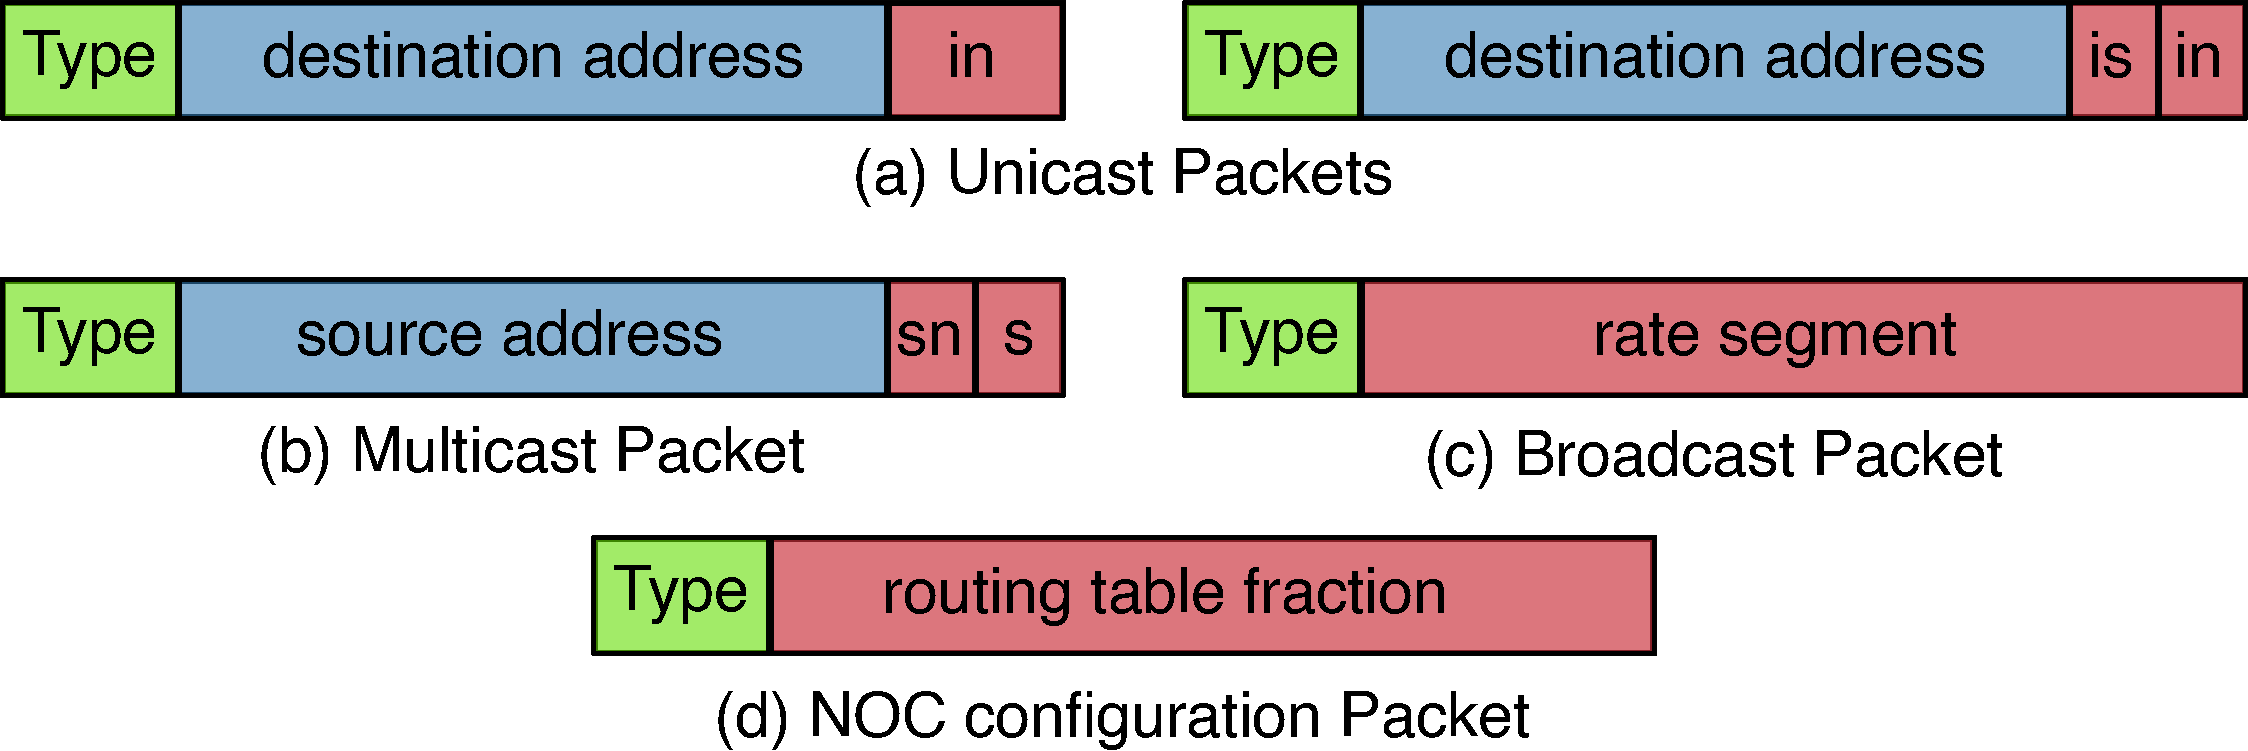
\includegraphics[width=0.75\columnwidth]{Figures/packet_format.pdf}
    \caption{Different packet formats to support network configuration and data communication.} 
    \label{figure:pktformat}
    \end{center}
    \vspace{-8mm}
\end{figure}